\documentclass[a4paper,12pt]{article}

\usepackage[english]{babel}
\usepackage[T1]{fontenc}
%\usepackage[latin1]{inputenc}	
\usepackage[utf8]{inputenc}	

%\usepackage{colortbl}
\usepackage[usenames,dvipsnames]{color} % for code listings
% Sequence diagrams
\usepackage[underline=true]{pgf-umlsd}
\usetikzlibrary{calc}
\usepackage[top=3cm, left=3cm, right=3cm, bottom=3cm]{geometry}								% marges

\usepackage{array,multirow,multicol,tabularx}		

\usepackage{amsmath,amssymb,mathrsfs}	
%\usepackage{mathtools}

\usepackage{soul}
%\usepackage{pifont}

\usepackage{multicol}

\usepackage{fancybox}

%\usepackage{epic, eepic}
\usepackage{graphicx}

\usepackage{float,picins}

\usepackage{hyperref}

\usepackage{listings}

\usepackage{ccaption}

\usepackage{pgf,tikz}
\usetikzlibrary{arrows}

\usepackage{thmbox}

\usepackage{placeins}

\usepackage{etex}

%\usepackage[ruled,vlined]{algorithm2e}

\usepackage{xspace}

\usepackage{graphicx}
\graphicspath{{images/}}

\hyphenation{TUM-Online}


\makeatletter

\newskip\@bigflushglue \@bigflushglue = -100pt plus 1fil

\def\bigcenter{\trivlist \bigcentering\item\relax}
\def\bigcentering{\let\\\@centercr\rightskip\@bigflushglue%
\leftskip\@bigflushglue
\parindent\z@\parfillskip\z@skip}
\def\endbigcenter{\endtrivlist}

\makeatother

%todo anfang
  \newcommand{\todo}[1]{
  % Add to todo list
  \addcontentsline{tdo}{todo}{\protect{#1}}
  %
  \begin{tikzpicture}[remember picture, baseline=-0.75ex]
      \node [coordinate] (inText) {};
  \end{tikzpicture}
  %
  % Make the margin par
  \marginpar{
      \begin{tikzpicture}[remember picture]
          \definecolor{orange}{rgb}{1,0.5,0}
   
          \draw node[draw=black, fill=orange, text width = 3cm] (inNote)
                   {#1};
      \end{tikzpicture}
  }
  %
  \begin{tikzpicture}[remember picture, overlay]
      \draw[draw = orange, thick]
          ([yshift=-0.2cm] inText)
              -| ([xshift=-0.2cm] inNote.west)
              -| (inNote.west);
  \end{tikzpicture}
  %
  }
% todo ende

% sonstige shortcuts:
\newcommand{\app}{\textit{GetInTUM}\xspace}

\newcommand{\be}{\textit{backend}\xspace}
\newcommand{\ph}{\textit{smartphone}\xspace}
\newcommand{\ter}{\textit{NFC terminal}\xspace}

\newcommand{\vows}{\textit{vows.js}\xspace}
\newcommand{\node}{\textit{Node.js}\xspace}
\newcommand{\mongo}{\textit{MongoDB}\xspace}

%________________________________________________________

\begin{document}

\noindent %
\begin{minipage}{0.5\textwidth}
\begin{flushleft}
	\begin{tabular}{lm{6cm}}
	\multirow{5}{*}{
\includegraphics[scale=1]{images/IN_logo.png}} \\
	 & Bj\"{o}rn Kirschner \\
	 & Sebastian Schleemilch \\
	 & Stefan Smarzly \\
	 & \\
	 & \\
	\end{tabular}
\end{flushleft}
\end{minipage}
\hfill
\begin{minipage}{0.5\textwidth}
\begin{flushright}
	
\includegraphics[scale=1]{images/tum_logo.png}
\end{flushright}
\end{minipage}

\begin{center}
{\LARGE\textbf{\textsc{GetInTUM - Door Access System}}}

\large \textit{Final Documentation for Android Practical Course (F13)} \\
\large \today
\end{center}

\bigskip
\bigskip

\hrule
\bigskip
\bigskip

\begin{bigcenter}
\begin{tabular}{cccc}
\includegraphics[height=3.4cm]{images/img_bjoern_small.jpg}&
\includegraphics[height=3.4cm]{images/img_sebastian_small.jpg}&
\includegraphics[height=3.4cm]{images/img_stefan_small.jpg}\\
Bj\"{o}rn Kirschner & Sebastian Schleemilch & Stefan Smarzly
\end{tabular}
\end{bigcenter}

\bigskip
\bigskip

\hrule
\bigskip
\bigskip


\bigskip

\textbf{Abstract:} blabla ... \todo{TODO!!!}

\newpage
\bigskip
\tableofcontents

\bigskip
\bigskip
\bigskip
\hrule

\bigskip
\bigskip

%\newpage

\section{Introduction}

This paper presents the final of \app, a solution to control access to university buildings via a mobile device communicating with a receiver at the door.
This communication works via near field communication (NFC).
Main contribution of the presented project is an Android application embedded in a holistic system which provides simple door access capabilities.
%Given the limited scope of the project, we start with a prototypical setup while striving for the system to eventually be employed by the TU München (TUM).

%Apart from this application we plan a prototypical implementation of a NFC reader using 



\subsubsection*{Problem description}

%\todo{ganzes Kap kürzen!}

Full-time students at TU München often face the problem that courses or seminars take place on a Saturday or a Sunday.
Since buildings at the university campus are generally closed at weekends, students have to ring for the security personnel to open the door.
But due to the number of students entering and leaving university buildings, door wardens hardly ever check the legitimacy of any entrant's business, i.e.~if they really are students.
This situation is unsatisfactory for all participants:

\begin{itemize}
\item Students needlessly have to wait for someone to open the door.
\item Door wardens get distracted from more important work.
\item Door wardens and university authorities cannot guarantee that entering people are students (or authorised persons in general).
\end{itemize}

\subsubsection*{Solution}

In order to overcome afore-mentioned problems, this paper presents a solution which allows students to authenticate at a door system and are granted or denied access automatically. This approach helps to...

\begin{itemize}
\item reduce possible waiting times for students,
\item unburden door wardens,
\item and guarantee that only students and other authorised persons are granted access.
\end{itemize}

A few areas in TUM buildings already use an access mechanism via the student card.
But for security reasons this student card solution is not ideal.
Because the card only identifies via an imprinted unique ID, reading and duplicating the card is possible.
For this reason we developed a smartphone solution which implements state of the art security mechanisms.
This solution has the potential to not only be used for main door entrances to the university but also to control access to chairs or other restricted areas.
It is an overall solution, relying solely on the user's smartphone.
 
 \subsubsection*{Structure of this paper}

The following chapter motivates the need for such a door access solution and sketches the project idea. Chapter \ref{sec:arch} then details the proposed technical architecture. Due to a several possible approaches, chapter \ref{sec:alt} justifies our design decisions. Finally, chapter \ref{sec:team} introduces all team members and chapter \ref{sec:plan} outlines a project plan.\todo{Anpassen} 

\section{Project Team}\label{sec:team}

\subsubsection*{Björn Kirschner}
%
\begin{minipage}{0.2\textwidth}
\begin{flushleft}
	\includegraphics[width=2.2cm]{img_bjoern_small.jpg}
\end{flushleft}
\end{minipage}
\hfill
\begin{minipage}{0.8\textwidth}
%
Graduated in Information Systems at TU München. Is currently studying Information Sciences with a focus on IT security. Hence, secure communication and protocol design of the door access solution proposed in this paper will be of particular interest to him.
%
\end{minipage}


\subsubsection*{Sebastian Schleemilch}
%
\begin{minipage}{0.2\textwidth}
\begin{flushleft}
	\includegraphics[width=2.2cm]{img_sebastian_small.jpg}
\end{flushleft}
\end{minipage}
\hfill
\begin{minipage}{0.8\textwidth}
%
Made his bachelor in Mechatronics at the FAU Erlangen-Nuremberg. Right now, he is studying Automotive Software Engineering at TUM in the third out of four semester. He is excited about the combination of software and the interaction with physical problems, which also explains his previous education steps so far.
Since this project will also be a mixture of pure software problems and the physical frontend (in this case: opening the door), Sebastian fits quite well into it.

\end{minipage}


\subsubsection*{Stefan Smarzly}
%
\begin{minipage}{0.2\textwidth}
\begin{flushleft}
	\includegraphics[width=2.2cm]{img_stefan_small.jpg}
\end{flushleft}
\end{minipage}
\hfill
\begin{minipage}{0.8\textwidth}
%
Graduated in Informatics at TU München. Currently, Stefan is studying Informatics in the Master program at TUM with an emphasis on Robotics, Distributed Networks and Security.
He is keen on working with Distributed Embedded Systems and to secure the communication between the devices.
This project provides ideal conditions to apply his knowledge about deploying a secure Distributed System that physically interacts with its environment.
%
\end{minipage}
\section{Action Planning and Scheduling}\label{sec:plan}

The Gantt chart in chapter gives a brief overview of all tasks done for the project.
It lists important milestones and tasks along with information about who of the three team members\footnote{In this context, `St' stands for `Stefan', `Se' for `Sebastian' and `Bj' for `Björn'} is mainly involved.

Most defined deadlines could be reached in time.
Some tasks could even be started earlier than expected, particularly the testing of communication to the backend (due to consequent test-driven development) and the integration of the backend into Android app and NFC terminal ($\rightarrow$ continuous integration).

Since we lingered a bit too long with vain attempts to integrate our solution into Mr.~Recksiegel's hardware (c.f.~section \ref{sec:project_flow}) some tasks were slightly behind schedule.
These hardware problems also had effects on subsequent tasks.
Delayed tasks are marked with yellow and orange lines in the Gantt chart.


\iffalse
The chart includes tasks since the start of the project.
These already finished steps focused on conceptual and organisational aspects.
Most importantly, we obtained approval of important TUM stakeholders:
\begin{itemize}
\item Mr.~Bernhofer from the TUM IT Management, responsible for identity management and connections to external IT systems. He provided us with information how to access central TUM services (Active Directory, Token management for TUMonline, ...).
\item Mr.~Recksiegel from the TUM physics department, who is the head behind an existing student card to NFC solution running in the physics building. He promised help with hardware issues and to finally push the integration of our smartphone to NFC solution into the already existing systems.
\end{itemize}
%Mr.~Recksiegel also mentioned another possible field of application: 
%die Duschen halt....
\fi





%\newpage



\par\vfill\break % Break Last Page

\advance\vsize by 6cm % Advance page height
\advance\voffset by -2cm % Shift top margin
% Start big page
\centerline{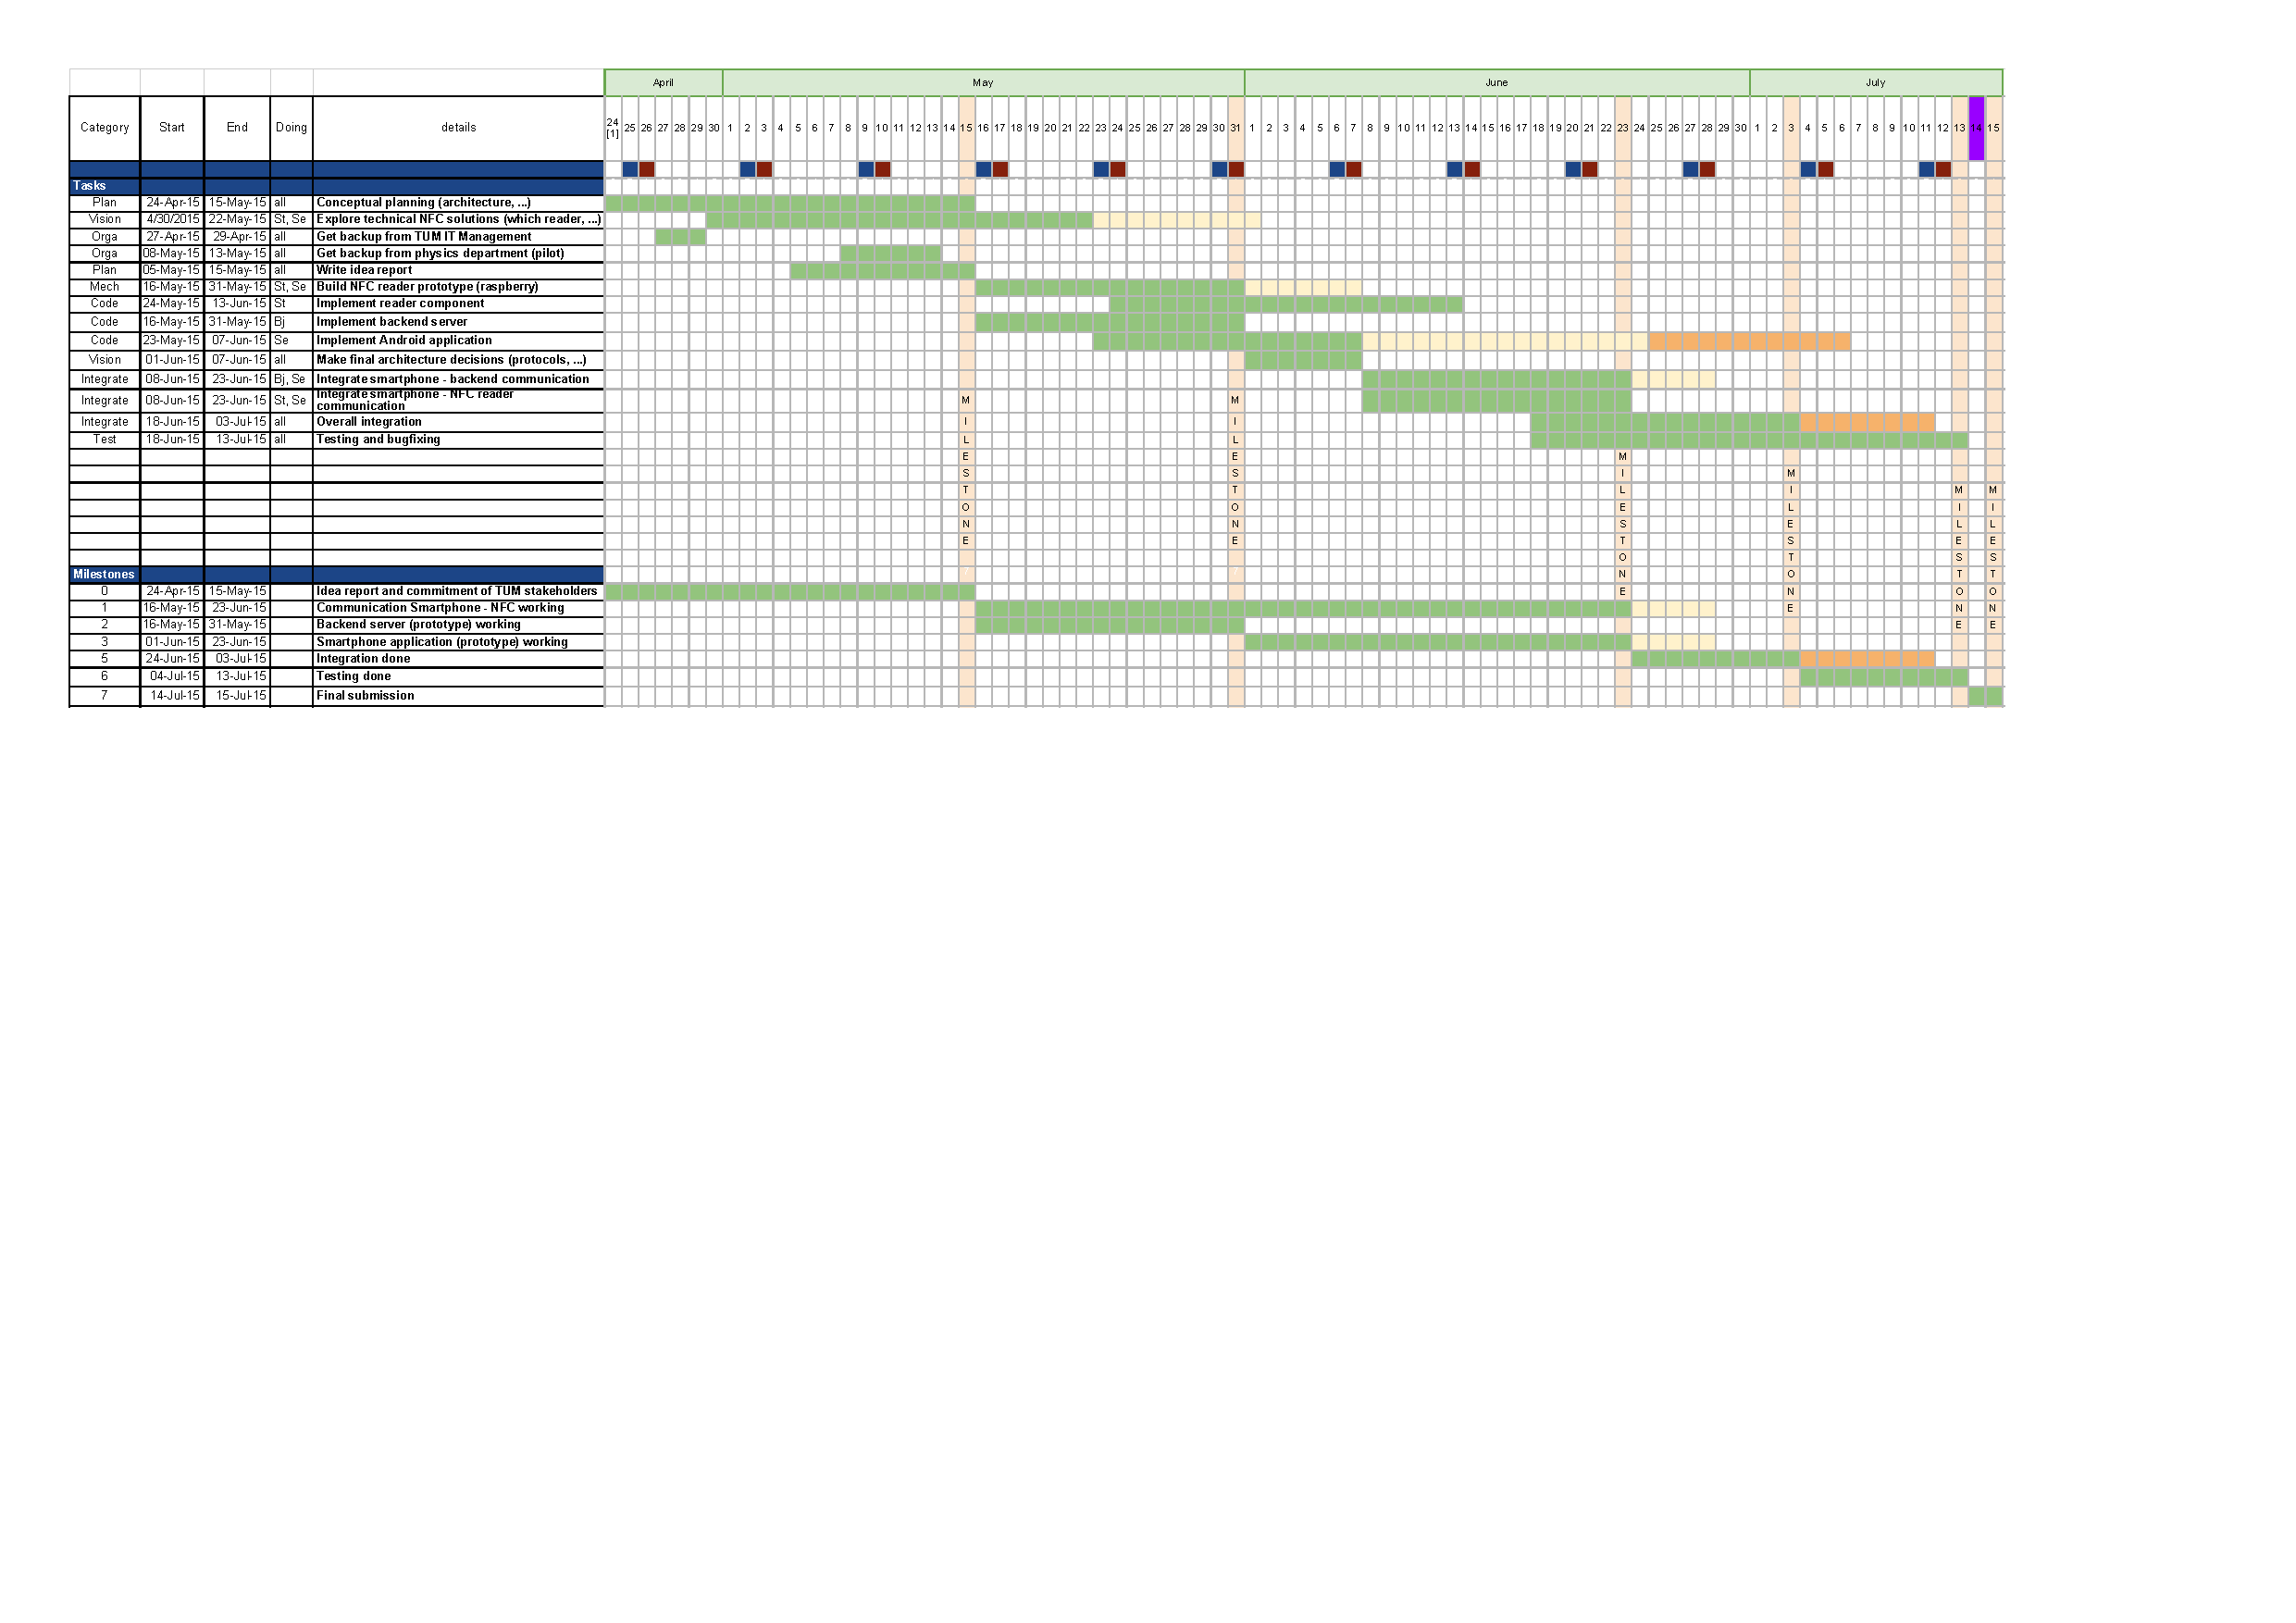
\includegraphics[height=79mm,angle=270]{gantt_final}}
% End big page
\par\vfill\break % Break the page with different margins

\advance\vsize by -6cm % Return old margings and page height
\advance\voffset by 2cm % Return old margings and page height
\section{Project Flow}\label{sec:project_flow}

Concerning the implementation of all planned functionality of \app we faced few obstacles.
Most issues of the initial project plan could be finalized smoothly.

In several details the functionality could even be improved by \textbf{additional features}.
The following list explains all important changes and new features:
\begin{itemize}
\item The smartphone app can now ask the backend if the user has already activated his token in TUMOnline.
This ensures that the smartphone does not constantly try to proceed with the next step (upload public key) but of course always fails because only activated user accounts are allowed to perform this task.
\item A user can now ask the backend to generate a new pseudo ID for him.
This effectively increases the user's privacy, as NFC terminals are no longer able to track his actions.
\item Users can now delete their accounts from the backend's database, which in general should be a useful feature.
\item ...?\todo{mehr?}
\end{itemize}

\bigskip


But as in most projects we also faced a few setbacks and \textbf{problems}.
Our original ambition was to see the \app solution employed in a real environment at TUM.
To accomplish this goal we had several meetings with Mr.~Bernhofer from the TUM IT Management and later with Mr.~Recksiegel from the TUM physics department.
The latter already runs several door terminals which allow registered users to enter rooms by holding their student cards to a NFC reader.
As we did not and still do not want to promote our solution as competition to the solution already employed in some rooms of the physics department, we searched for a way to integrate \app into the existing system of the TUM physicists.
For several reasons this turned out to be more difficult than expected.
\begin{itemize}
\item TUM student cards communicate via NFC standards from the company LEGIC, which are not compatible with the NFC standards that Android smartphones understand.
\item The NFC reader built into the TUM physics solution is not able to communicate via NFC standards other than LEGIC.
\item Since the NFC reader used by the TUM physics department is a proprietary product and ships with a rather small housing, we did not manage to easily mount a second NFC antenna into this housing.
\item Integrating two different NFC readers into the door terminal entailed several physical problems.
For two NFC readers to function independently they would need to be mounted with at least about five centimetres distance to each other.
This led to concerns that a terminal with two distinct NFC readers might not be intuitive for users.
\item Diese Liste muss in Details noch überarbeitet werden!\todo{!!!}
\item Ist not etwas wirr und unstrukturiert...
\item ...hab ich was vergessen?\todo{???}
\end{itemize}


% -------------- Kommentare und alter Mist ----------------------- %
\iffalse

:\todo{TODO}
hatten wir ja ein paar: Zusammenspiel mit anderen Lesegeräten (Legic), ...
-> dadurch: unwahrscheinlicher, dass die Lösung in der Praxis eingesetzt werden wird.

any problems? Differences to the planned functionality?

Differences to the planned functionality:
gibt's bei uns eher nicht, oder?

Stefan: Ne, eigentlich sogar noch mehr Funktionalität und erhöhte Sicherheit/Anonymität als spezifiziert.
\fi
\section{Architectural Overview}\label{sec:arch}

\todo{jetzt: project description}

\todo{total umschreiben}

The basic architecture to develop the system outlined above will consist of the following parts:

\begin{itemize}
\item The smartphone, including a NFC chip as well as an internet connection to register with the service.
An internet connection will only be needed once during initialization of the system or when creating a new key pair in case of revocation.
The smartphone must also be able to create an asymmetric key pair and securely store it persistently.
\item The Door Access System, also including a NFC chip which can send and receive.
A simple NFC reader would not suffice as it would be vulnerable to simple replay attacks.
The door system also needs access to the internet or at least to an intranet in order to check if the student or the employee has access to the specific area and to get other information for realizing security features like encryption of the communication. Therefore, some kind of computer is also needed, interacting with the NFC hardware as well as with the back-end.
%would not be enough due to simple replay attacks. The Door Access System also needs access to the internet or at least to an intranet to check if the student or the employee has access to the specific area and to get other information for realizing security features like encryption of the communication. Therefore, some kind of computer is needed, interacting with the NFC hardware as well as with the back-end.
\item A back-end system, which will check student ID, the corresponding TUMOnline token and will fetch the generated public key from the smartphone. It will finally store the public key of every registered student.

\item The TUMOnline system, which has enrolment information about every student and can confirm the status of a person.
\end{itemize} 
%
The following figure gives a holistic overview of the basic architecture (based on public-key cryptography as discussed in section \ref{sec:alt:proto:pubkey}): \newline
 \begin{center}
	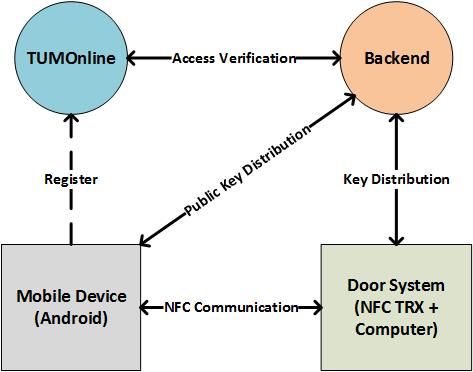
\includegraphics[scale=1]{basic_architecture.jpg}
\end{center}


\subsection{Registration with Back-end}
To initialize the system, the user has to contact the back-end system once for authentication.
% by providing his user ID.
The user provides his ID along with the user token that is generated by TUMOnline.
%To activate the user token that is generated by TUMOnline, the user has to login separately on a web platform. 
The back-end system can check if the proposed access token of the user is valid or not via the TUMOnline Webservice API.
%For that purpose, the connection to the TUMOnline service is needed to get this kind of information.
If the user has sent the right access token, the back-end system will demand the public part of the user's asymmetric key pair (which has been created on the user's smartphone before starting the communication).
In this step, the server will take particular care that the authentic user is in possession of the private part of the transmitted public key and doesn't pretend to be a different identity.
%create a public key pair and will send the user his private key. Therefore, a key storage and management system has to be implemented.
All connections to the back-end are planned to be secured by TLS.


\subsection{Authentication between Smartphone and NFC Transceiver}
After the user has registered with the back-end system, he can communicate with the NFC reader. 
A three-way handshake assures a secure connection between smartphone and NFC reader.
In order to verify the soundness of the procedure, in particular the authenticity of the communication partner, the NFC reader (i.e.~the system behind it) will fetch the public key of the user who wants to authenticate from the back-end system.
Furthermore, the Door Access System will check if the user has access to the requested area.
It will finally unlock the door if all checks were positive.

%\section{Design Alternatives}\label{sec:alt}

\subsection{NFC Communication}\label{sec:comm}
NFC devices are typically specified for a maximum range of $10cm$. Therefore, other solutions incorporating NFC assume that the physically constrained range is enough to prevent attackers to tamper with the transmitted data.
As basic NFC hardware is quite cheap, this is probably not the right approach for the future.

A fundamental part of our \app entrance access solution is the secured NFC communication between a mobile device and a terminal installed at a gate.
This section presents building blocks ranging from low-level to high-level aspects of the NFC communication in order to achieve this goal.


\subsubsection{Hardware Setup}
Exchanging data needs a communication link between an Android smartphone and a NFC terminal.
To make it work, the NFC unit must support common NFC standards (e.g., ISO/IEC 14443) and provide stable transmission properties on the data-link layer.
Therefore, we examine our utilized hardware setup. Figure \ref{fig:nfc:hw} shows our prototype interfacing with a mobile device.
%
\begin{itemize}
	\item Raspberry Pi with a PN532 compliant NFC cape, e.g., \textit{ITEAD PN532 NFC module}.
	\item Android mobile device with NFC capabilities and Android 4.4 or newer.
\end{itemize}
%
\begin{figure}[h]
    \centering
    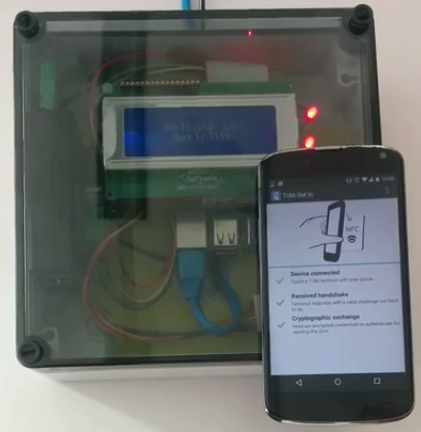
\includegraphics[width=.4\linewidth]{nfc_hardware}
    \caption{NFC hardware. Below the smartphone, there is the NFC cape that successfully finished the authentication with the smartphone.}
    \label{fig:nfc:hw}
\end{figure}
%
Using the Raspberry Pi as underlying platform and the proposed NFC transceiver, a cheap and powerful setup is possible.
It provides a rich interface to interact with the environment and allows an easy integration into existing door electronics.
For the basic operation, the free NFC library \textit{libnfc}\footnote{\url{http://nfc-tools.org/}} abstracts elementary low-level functionality like modulations for ISO/IEC 14443 standard.
It is a building block to establish a simple data-link layer for \app.

The counterpart of the terminal is a smartphone with NFC transceiver and Android 4.4 (or higher versions) that offers basic APIs to exchange data with other NFC enabled devices like our NFC cape.

\subsubsection{Low-Level Communication and Message Fragmentation}
% Card Emulation on Android side
% Terminal behaves as reader
Still, for our approach, we cannot rely on high-level APIs like Android Beam(R), for instance.
At the time of this report, it effectively only allows an one-directional communication link. The same holds for the available high-level APIs of NDEF Push.
In our case, we need a mutual authentication. This requires a bi-directional communication link.
\\
Therefore, the following architecture is used:
\begin{itemize}
	\item Android phone with Host-based Card Emulation: emulates a card based on NFC-Forum ISO-DEP specification (ISO/IEC 14443-4 in our case).
	\item NFC terminal: acts as a compliant NFC reader.
\end{itemize}
%
Given the activation, anti-collision (layer 3) and transmission properties (layer 4) are primarily managed by Android and \textit{libnfc}, an enhanced version of ISO 7816-4 layer is deployed to organize the data exchange.
It uses APDU headers to specify the type and size of data, i.e., whether the reader sends some (outgoing) chunks of data or expects the mobile device to response with some (incoming) data.

This also is the place where message fragmentation comes in.
Layer 4 can transmit messages with a maximum size of $256$ bytes.
APDU headers and status codes already consume between 2 and 5 bytes. As RSA encryption with 2048 bit alreday requires the same amount of bytes for the ciphertext, our implementation brakes down the messages into chunks with a maximum size of $125$ bytes.
According to some tests, this ensures a stable connection between the devices.
The control flow is controlled by specifying the remaining data size in the APDU status fields.

%\subsubsection{Protocols for Authentication between Smartphone and NFC Reader}\label{sec:alt:proto}
%A critical aspect in our project is the communication between a smartphone $ S $ and the NFC component $ T $.
%It is important that it is safe so that no unauthorized party can easily gain access or eavesdrop sensitive information like the student ID.
%By placing the reader's antenna in the inner side of the door, it should be safe from physical threats from outside.
%To ensure a secure communication on top of the data carrier, we plan to use one of the protocols introduced in this section.
%Which one to finally choose depends on multiple aspects like the capabilities of the NFC hardware (e.g.~processing power), Android support or fault tolerance. This needs some testing done during the project. 

\subsubsection{Protocol with Public-Key Cryptography}\label{sec:proto:pubkey}
On the top level, the communication protocol relies on a local Public Key Infrastructure to establish secure communication links between the NFC participants.
For authentication on both sides and mitigation of several attack scenarios, it uses some ideas of the Needham-Schroeder-Lowe Public Key protocol. Lowe contributes an important security fix we use.
The scheme is enhanced to provide further security features specific for the utilized backend and the scenario.

%%%%%%%%%%%%%%%%%%%%%%%%%%%%%%%%%%%%%%%%%%%%%%%%%%%%%%%%%%%%%%%%%%%%%%%%%%%
% Redefine the \mess due to problems with math support $ \some_function $ %
% See: http://tex.stackexchange.com/questions/164707/how-to-use-greek-    %
%      letters-in-pgf-umlsd-or-generally-terms-starting-with              %
%%%%%%%%%%%%%%%%%%%%%%%%%%%%%%%%%%%%%%%%%%%%%%%%%%%%%%%%%%%%%%%%%%%%%%%%%%%
\renewcommand{\mess}[4][0]{
  \stepcounter{seqlevel}
  \path
  (#2)+(0,-\theseqlevel*\unitfactor-0.7*\unitfactor) node (mess from) {};
  \addtocounter{seqlevel}{#1}
  \path
  (#4)+(0,-\theseqlevel*\unitfactor-0.7*\unitfactor) node (mess to) {};
  \draw[->,>=angle 60] (mess from) -- (mess to) node[midway, above]
  {#3};
}
%
\begin{figure}[h]
	\begin{sequencediagram}
		\newinst{S}{Smartphone $ S $}
		\newinst[8.5]{T}{NFC Terminal $ T $}
		% \newinst[4]{rnc}{RNC}
		\mess{S}{1. $ {\{r_S, pseudoStudentID\}}_{K_{T-pub}} $}{T}
		\postlevel
		\mess{T}{2. $ {\{r_S, r_T\}}_{K_{S-pub}} $}{S}
		\postlevel
		\mess{S}{3. $ {\{r_T, H(salt|studentToken), commands\}}_{K_{T-pub}} $}{T}
		%\mess{nodeb}{Synchronization Indication}{rnc}
		%\filldraw[fill=black!30] ($(RRC Connection Setup to)+(0,-.3)$) rectangle ($(Synchronization Indication from) +(0,.3)$)
		%node[midway] {L1 Synchronization};
	\end{sequencediagram}
	\caption{Protocol design for secured communication between NFC terminal and mobile device.}
	\label{fig:nfc:protocol}
\end{figure}
%
\noindent
Figure \ref{fig:nfc:protocol} describes our proposed protocol.
Explanations:
%
\begin{enumerate}
	% 1.
	\item $ S \rightarrow T $:
	\begin{itemize}
		\item $ S $ generates a random number $ r_S $ and sends it to $ T $ together with the $ pseudoStudentID $, encrypted with the terminal's public key $ K_{T-pub} $. These keys are statically embedded in the Android application.
		\item The official student ID is replaced by the pseudonym $ pseudoStudentID $, which is associated with the official ID of the student in the backend.
		Like this, a MITM attack would not allow to directly gain information about the requesting person's ID.
		Furthermore, this pseudonym association can be changed regularly and at user's will.
	\end{itemize}	
	% 2.
	\item $ S \leftarrow T $:
	\begin{itemize}
		\item The terminal $ T $ looks up the public key $ K_{S-pub} $ for the pseudo student ID in the backend. If it doesn't exist, further communication stops here.
		\item On success, $ T $ generates a random number $ r_T $ and sends it back to $ S $ together with $ r_S $, encrypted with the user's public key $ K_{S-pub} $.
%		\item Providing the identity $ T $, the requesting party can verify whether the reader's public key changed. This could originate from an attack in step 1 (e.g., fake reader). In that case, abort further communication to assure confidentiality.
	\end{itemize}	
	% 3.
	\item $ S \rightarrow T $:
	\begin{itemize}
		\item If $ S $ receives a valid answer in step 2, it should be fine to proceed.
		\item $ S $ sends $ r_T $, a salted SHA-256 hash of $ studentToken $ and data to $ T $, encrypted with $ K_{T-pub} $.
		\item Having exchanged the random secrets $ r_S $ and $ r_T $ protected by the PKI, the communicating participants can be sure that these are fresh and authentic messages. Additionally, the public keys can only be fetched knowing the pseudo ID. To update a user's public key in the backend, it is necessary to sastify further conditions: secret token in addition to the real TUM student ID has to be known and the associated token must be active in TUMonline albeit a valid entry in TUM's active directory service.
		\item Salted SHA-256 student token $ H(salt|studentToken) $: as the random salt is unique per user and only known to the backend and the Android client, the terminal does not touch critical data.
		Still, by comparing the hash values received by the backend on retrieval of the user's public key, and the one sent by the smartphone in this step, the identity of the user is indirectly proven.
	\end{itemize}
\end{enumerate}
\section{Implemented Functions}\label{sec:functions}

Ph: smartphone
BE: backend server
Ter: NFC terminal
TuO: TUMOnline
TuAD: TUM Active Directory

\bigskip

All functions follow the general workflow.

\bigskip

passt das in dieser Form?\todo{???}

\noindent
\begin{tabularx}{\textwidth}{ l X c X } 
Components & Function & Planned & Implemented \\ \hline\hline


Ph $\rightarrow$ BE & Register user TUM ID and ask for a new token & \checkmark & \checkmark \\ 
BE $\rightarrow$ TuO & Request new token & \checkmark & \checkmark \\ 
BE & Store user data in a database & \checkmark & \checkmark \\ 
Ph $\rightarrow$ BE & Ask if new token has been activated &  & \checkmark (added to avoid vain attempts of following steps) \\ 
BE $\rightarrow$ TuO & Ask if new token has been activated & \checkmark & \checkmark \\ 
Ph & Generate asymmetric key pair & \checkmark & \checkmark \\ 
Ph $\rightarrow$ BE & Send public key to server & \checkmark & \checkmark \\ 
BE & Generate pseudo ID for user & \checkmark & \checkmark \\ 
Ph $\rightarrow$ BE & Renew pseudo ID and salt &  & \checkmark (to improve privacy) \\ 
Ph $\rightarrow$ BE & Remove user account &  & \checkmark \\ \hline


Ter $\rightarrow$ BE & Ask for public key corresponding to a pseudo ID & \checkmark & \checkmark \\
Ter $\rightarrow$ BE & Ask for salted hash of user token to a pseudo ID & & \checkmark \\
Ph $\rightarrow$ Te & Additional security layer by comparing hashed token both for BE and Ph. &  & \checkmark \\ 
BE $\rightarrow$ TuAD & Ask for student status & \checkmark & \checkmark (changed from $\rightarrow$ TuO to $\rightarrow$ TuAD for precision) \\ 
\end{tabularx}
\section{Test Plan}\label{sec:test_plan}

%\todo{struktur!}
%Test coverage, Test methods, Test responsibilities
%...Das Ganze auf den Funktionen aus den letzten Kapiteln basieren lassen....\\


Due to the strict separation of the components \be, \ph and \ter testing could partly be initiated in early stages of the project.

Particularly the \be component was required to quickly reach a robust state because both other components heavily rely on its functioning.
In order to guarantee this robustness, development followed a test-driven approach from the beginning.
Functionality required in the \be was first defined in a specifications document.
Subsequently test cases based on these specifications were written using \vows\footnote{Vows: Asynchronous behaviour driven development for Node. http://www.vowsjs.org}.
Only then did we begin to actually implement the defined functionality.

\medskip

\noindent
For testing all interfaces to and from the backend you may also refer to the specifications document ($spec.txt$) which lists all possible server messages, including all possible responses to potential expected and unexpected errors.

\bigskip

\noindent
High-level testing of the entire \app solution was done by using three different scenarios:
\begin{itemize}
\item A user has a valid TUMOnline account and is student.
\item A user has a valid TUMOnline account but is not student any longer.
\item A user has no valid TUMOnline account.
\end{itemize}

\noindent
On a low level, we tried to cover all possible causes of errors or unexpected behaviour.
Testing included:
\begin{itemize}
\item Trying requests with wrong or missing arguments.
\item Sending broken or incomplete packets.
\item Interrupting connections.
\item Testing with expected error messages of involved systems.
E.g.~TUMOnline may send an error message if a user has reached his token limit (10).
\item Testing possible unexpected failures of involved systems like connection problems to TUMOnline or the Active Directory.
\end{itemize}


\app's global test plan is based upon the high-level scenarios defined above and the list of functionality presented in chapter \ref{sec:functions}. It looks as follows:
\bigskip

\noindent
\begin{tabularx}{\textwidth}{ X X X c } 
Test case & Expected result & Result & OK? \\ \hline\hline

Ph $\rightarrow$ BE: Register with valid TUM ID & BE returns token, pseudo ID and salt & $\rightarrow$ BE returns token, pseudo ID and salt & \checkmark \\ 
 &  & $\rightarrow$ BE returns error & $\times$ \\ 
 &  & $\rightarrow$ No answer & $\times$ \\ 
 &  & $\rightarrow$ BE or Ph crash & $\times$ \\ \hline

Ph $\rightarrow$ BE: Ask if token is activated & BE returns $true/false$ & $\rightarrow$ BE returns $true/false$ & \checkmark \\ 
 &  & $\rightarrow$ BE returns error & $\times$ \\ 
 &  & $\rightarrow$ No answer & $\times$ \\ 
 &  & $\rightarrow$ BE or Ph crash & $\times$ \\ \hline

Ph $\rightarrow$ BE: Send $K_{pub}$ & BE returns OK & $\rightarrow$ BE returns OK & \checkmark \\ 
 &  & $\rightarrow$ BE returns error & $\times$ \\ 
 &  & $\rightarrow$ No answer & $\times$ \\ 
 &  & $\rightarrow$ BE or Ph crash & $\times$ \\ \hline

Ph $\rightarrow$ BE: Renew pseudo ID and salt  & BE returns new pseudo ID and salt & $\rightarrow$ BE returns new pseudo ID and salt & \checkmark \\ 
 &  & $\rightarrow$ BE returns error & $\times$ \\ 
 &  & $\rightarrow$ No answer & $\times$ \\ 
 &  & $\rightarrow$ BE or Ph crash & $\times$ \\ \hline

Ph $\rightarrow$ BE: Remove user account & BE returns OK & $\rightarrow$ BE returns OK & \checkmark \\ 
 &  & $\rightarrow$ BE returns error & $\times$ \\ 
 &  & $\rightarrow$ No answer & $\times$ \\ 
 &  & $\rightarrow$ BE or Ph crash & $\times$ \\ \hline

\end{tabularx}

\bigskip
\noindent
\begin{tabularx}{\textwidth}{ X X X c } 
Test case & Expected result & Result & OK? \\ \hline\hline

Ter $\rightarrow$ BE: Ask for $K_{pub}$ of a pseudo ID & BE returns $K_{pub}$, H(token) and salt & BE returns $K_{pub}$, H(token) and salt & \checkmark \\ 
 &  & $\rightarrow$ BE returns error & $\times$ \\ 
 &  & $\rightarrow$ No answer & $\times$ \\ 
 &  & $\rightarrow$ BE or Ter crash & $\times$ \\ \hline


\end{tabularx}

\bigskip
\noindent
\begin{tabularx}{\textwidth}{ X X X c } 
Test case & Expected result & Result & OK? \\ \hline\hline

Enter no ID at step 1 & Please enter ID message & as we expected & \checkmark \\ 
Enter non existent ID at step 1 & Wrong ID message & as we expected & \checkmark \\ 
Enter real ID & Backend connection and forwarding to step 2 & as we expected & \checkmark \\ 
Swipe through pages without entering an ID & Display status correctly at all times & as we expected & \checkmark \\ 
Open/resume app & crosscheck user status with backend and display the appropriate page & as we expected& \checkmark \\ 
Resume app after token activation & update step 2 and forward the user to register complete & as we expected & \checkmark \\ 
Delete token by hand, resume to app & pages need to be updated properly, user gets forwarded to step 1 & as we expected & \checkmark \\ 

Select settings menu at any time & open settings page & rarely sporadically, the app crashes & $\times$ \\ 
\end{tabularx}




%-------- from Wikipedia: -----------------
\iffalse
IEEE 829-2008, also known as the 829 Standard for Software Test Documentation, is an IEEE standard that specifies the form of a set of documents for use in defined stages of software testing, each stage potentially producing its own separate type of document.[1] These stages are:

Test plan identifier
Introduction
Test items
Features to be tested
Features not to be tested
Approach
Item pass/fail criteria
Suspension criteria and resumption requirements
Test deliverables
Testing tasks
Environmental needs
Responsibilities
Staffing and training needs
Schedule
Risks and contingencies
Approvals
\fi

\section{Conclusion}\label{sec:conclusion}


Outlook?

- Can be adapted for more advanced rules. Do more fine-grained access control. E.g. doors at chair X only open if someone from chair X is allowed to.

- Die Lösung im Zusammenspiel mit dem Legic-Zeugs beschreiben. Das mit zwischen den zwei Readern hin- und herschalten.
Wobei Teile dieser Problembeschreibung schon ins Kapitel ``project flow'' müssen.

- Könnte man in die TUM-Campus-App integrieren...

- Was man in der Praxis machen müsste: halbfertige Registrierungen (Token nicht aktiviert) nach einiger Zeit wieder aus dem Backend löschen. Sonst könnte jemand das Backend total zumüllen. DoS-mäßig...

- Natürlich müsste man das Backend irgendwo auf einem TUM-Server hosten und neue Zertifikate verwenden (von der TUM ausgestellt und signiert).

- (eventuell) Man müsste IP-Adressen von requests im backend loggen. Sonst könnte man mittels Backend als Proxy TUMOnline spammen.
\section{Tutorial}\label{sec:tutorial}

Before actually using the \app solution on a smartphone, both the \be and a \ter have to be running.
Hence this chapter starts with installation instructions for \be and \ter.

General note: a command line starting with \# indicates a root shell, a \$ symbol indicates one without super-user privileges.

\subsection{Install and Launch Backend Server}

The server was implemented based on the JavaScript (JS) technologies \node and \textit{ME(A)N.js} (M = \mongo, E = $express.js$ [web server], A = $angular.js$ [currently not used], N = \node).
Hence it requires a running \mongo database and \node to be installed.
This chapter serves as a recommendation for starting the server.
Experienced users may also install some components locally (without the $-g$ option) or omit some parts.\medskip\\
1.) Install \node.\smallskip\\
2.) Install $npm$, the Node Package Manager.\smallskip\\
3.) Download \mongo.\smallskip\\
4.) Start \mongo via
\begin{lstlisting}
   $ <path-to-mongodb>/bin/mongod
\end{lstlisting}
5.) Install $bower$, a package manager.
\begin{lstlisting}
   # npm install -g bower
\end{lstlisting}
6.) Install $grunt$, a JS task runner for automation.
\begin{lstlisting}
   # npm install -g grunt-cli
\end{lstlisting}
7.) Install $vows$, a JS framework for writing and executing test suites. This is only necessary if tests need to be run.
\begin{lstlisting}
   # npm install -g vows
\end{lstlisting}
8.) Install all \node dependencies of the \be server. $npm$ automatically loads all dependencies defined in $package.json$ and stores them locally.
\begin{lstlisting}
   $ npm install
\end{lstlisting}
9.) Finally, \textbf{run the server} via the $grunt$ client (optionally with the environment variable \textit{NODE\_ENV=test}).
\begin{lstlisting}
   $ grunt
\end{lstlisting}\bigskip
(10.) Optionally, run the $vows$ test suite (change to $/test$ directory first; \textit{NODE\_ENV=test} is required for some unit tests).
\begin{lstlisting}
   $ vows interfaces-test.js --spec
\end{lstlisting}

\subsection{Install and Launch NFC Terminal}
Install the necessary components by issuing the following command on a Raspberry Pi:
\begin{lstlisting}[breaklines=true]
   # apt-get install libusb-dev build-essential autoconf2.64 libtool python3 gettext libreadline-dev
\end{lstlisting}
%
First, install libnfc in the following manner:
\begin{lstlisting}[breaklines=true]
   $ cd ~
   $ git clone https://github.com/nfc-tools/libnfc.git
   $ cd libnfc
   $ # Compilation
   $ autoreconf -vis
   $ ./configure --sysconfdir=/etc --with-drivers=pn532_spi
   $ make
   # make install
\end{lstlisting}
Copy the sample configuration file to the system location:
\begin{lstlisting}[breaklines=true]
   # mkdir /etc/nfc
   # cp libnfc.conf.sample /etc/nfc/libnfc.conf
\end{lstlisting}


%
Edit the content of the configuration file. The relevant lines should be configured as follows:
\begin{lstlisting}[breaklines=true]
allow_autoscan = true
log_level = 2
device.name = "itead_pn532"
device.connstring = "pn532_spi:/dev/spidev0.0:500000"
\end{lstlisting}
%
Install pyNFC (\url{https://github.com/grandcat/pynfc}) for Python 3 as described in its \texttt{README.md}.

\todo{Finish}

%cd ~git d
%git clone https://github.com/grandcat/tum_getin.git
%
%sudo apt-get install python3-crypto
%
%libnfc:
%wget https://libnfc.googlecode.com/files/libnfc-1.7.0.tar.bz2
%tar -jxvf libnfc-1.7.0.tar.bz2
%cd libnfc-1.7.0 
%./configure --prefix=/usr --sysconfdir=/etc --with-drivers=pn532_uart,pn532_spi,pn532_i2c 
%make install all 
%
%git clone https://github.com/ikelos/pynfc.git
%cd pynfc/src	
%2to3 -w nfc.py
%
%mv nfc.py ~/tum_getin/code/nfcTerminal/PyNfcTerminal
%cd ~/tum_getin/code/nfcTerminal/PyNfcTerminal
%
%python3 main.py




%\iffalse
%\bigskip
% -------------------------------------------------------------------
%[language={[x86masm]Assembler}, escapeinside={(*§}{§*)}, basicstyle=\ttfamily\scriptsize, caption={blablabla}, label={lst:1}]
\begin{lstlisting}
# npm install -g bower
# npm install -g grunt-cli
# npm install -g vows		(optional; runs unit tests)
$ npm install
\end{lstlisting}
%\bigskip

%\fi


\subsection{Use the GetInTUM Android Application}
\begin{enumerate}
   \item The first app start will show the following page:
   \begin{figure}
   \centering
   \begin{minipage}{.5\textwidth}
     \centering
     
\includegraphics[width=.4\linewidth]{RegisterStep1}
     \caption{A figure}
     \label{fig:test1}
   \end{minipage}%
   \begin{minipage}{.5\textwidth}
     \centering
     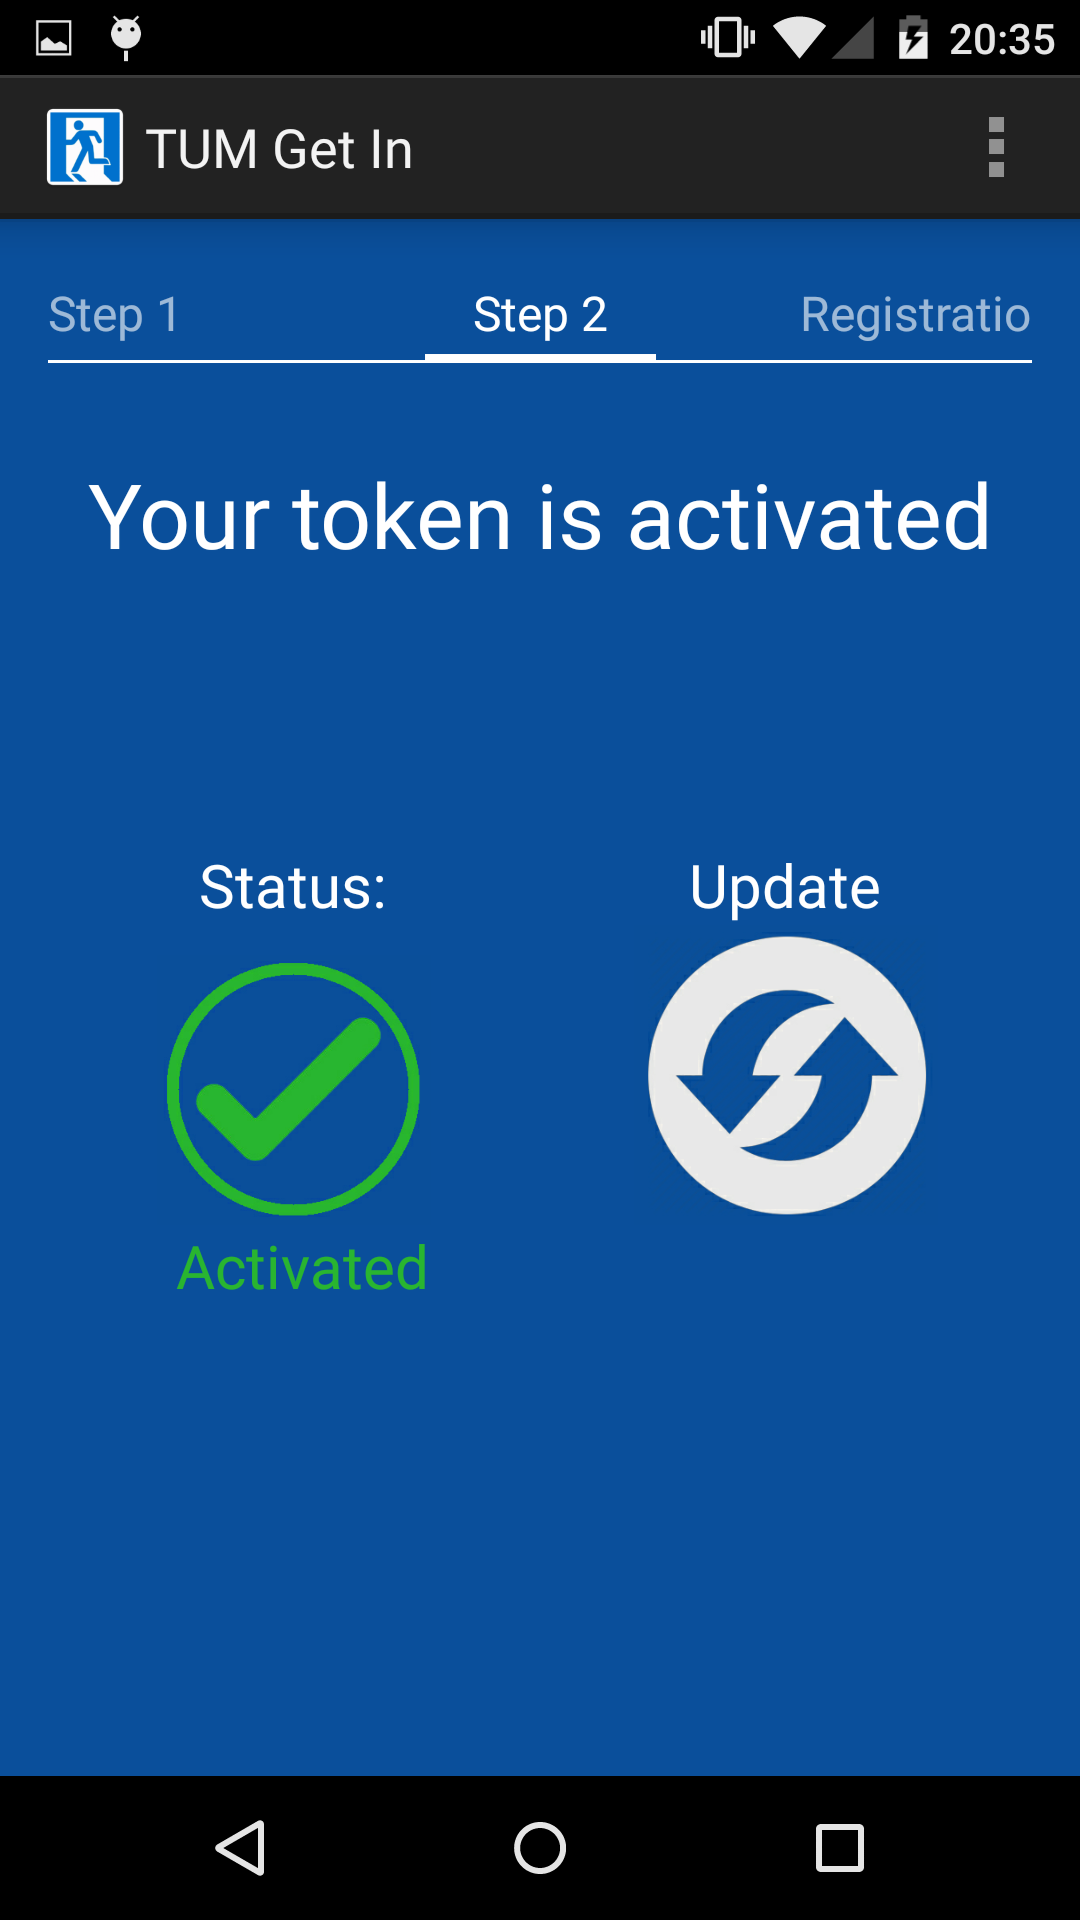
\includegraphics[width=.4\linewidth]{RegisterStep2_Activated}
     \caption{Another figure}
     \label{fig:test2}
   \end{minipage}
   \end{figure}

\end{enumerate}

\end{document}
